\documentclass{szzclass}
\usepackage{hyperref}
\usepackage{longtable}
\usepackage{booktabs}

\subject{DBS}
\code{BI-WSI-SI-03}
\topic{Pokročilé principy dotazování v SQL: agregace, vnější spojení, vnořené dotazy, všeobecná kvantifikace.}
\providecommand{\tightlist}{%
  \setlength{\itemsep}{0pt}\setlength{\parskip}{0pt}}

\begin{document}
\tableofcontents
\newpage

\section{Agregace}
Výpočet napříš skupinou zdrojových řádků. Syntax:
\begin{itemize}
    \item agregační\_funkce({\underline{ALL}|DISTINCT} sloupec | vyraz)
    \begin{itemize}
        \item COUNT, SUM, MAX, MIN, AVG\dots
        \item COUNT($\oslash$) = 0
    \end{itemize}
\end{itemize}
\begin{figure}[h!]
    \centering
    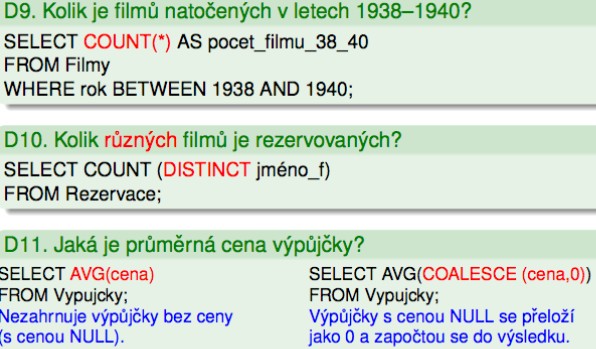
\includegraphics[width = 0.8 \textwidth]{topics/bi-wsi-si-04/images/agregation.png}
    \caption{Úkázka agregační funkce}
\end{figure}
Pořadí vyhodnocení:
\begin{itemize}
    \item zdroj - from
    \item selekce - where
    \item seskupení - group by
    \item agregační funkce
    \item selekce na výsledky agregační funkce - having
    \item řazení výsledků - order by
\end{itemize}
\section{Vnořené dotazy}
Dělí se na vztažné a nevztažné.
\begin{itemize}
    \item vztažné - použivají referenci na nadžazený dotazování (většinou časově náročnější)
    \item nevztažné - jedná se o nezávislý poddotaz, který nemá vztah s nadřazeným
\end{itemize}
\section{Pohledy - view}
\begin{itemize}
    \item pohled je virtuální relace
    \item je uložen ve formě SELECT příkazu
    \item z hlediska dotazování zaměnitelný s tabulkou
    \item nepřinášejí výkonové zrychlení - k tomu lze použít Materialized views
\end{itemize}

\section{Vnější spojení}
Vnější spojení (outer join) - normální spojení (inner join) + lefá/pravá/obě (left/right/join). Chybějící sloupce jsou doplněny
hodnotou NULL.
\newline
anti-join - redukce n-tic relace za ty, které nejsou spojitelné s žádnou n-ticí druhé relace
\begin{figure}[h!]
    \centering
    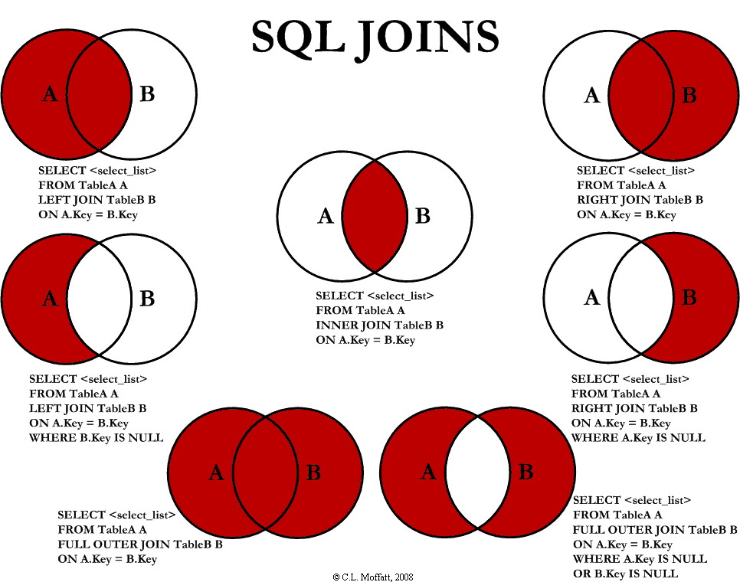
\includegraphics[width = 1 \textwidth]{topics/bi-wsi-si-04/images/sqlJoin.png}
    \caption{Přehled join příkazů}
\end{figure}

\section{Kvantifikátory}
Existenční (exists / not exists) vs všeobecný (není přímo implementován)
\newline
Exists:
\begin{itemize}
    \item nezáleží na tom, co se vybere ve vnořeném selectu
\end{itemize}
\begin{figure}[h!]
    \centering
    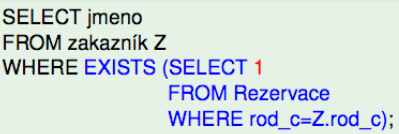
\includegraphics[width = 0.6 \textwidth]{topics/bi-wsi-si-04/images/exists.png}
    \caption{Úkázka exists}
\end{figure}
\begin{figure}[h!]
    \centering
    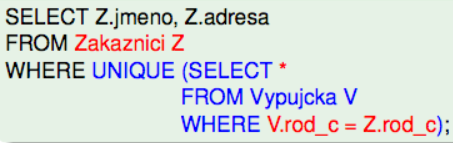
\includegraphics[width = 0.6 \textwidth]{topics/bi-wsi-si-04/images/unique.png}
    \caption{Úkázka unique}
\end{figure}
\begin{itemize}
    \item unique při vrácení prázdné množiny vrací true
    \item exists vrací false
\end{itemize}
\end{document}